We applied our feature extraction code first to the 120 images giving us the distribution of the ratings as seen on \ref{fig:Automatic feature extraction}:

\begin{figure}[H]
    \centering
    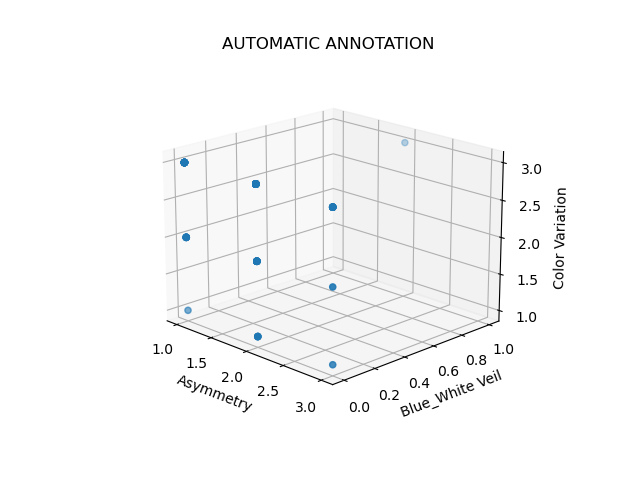
\includegraphics[width=1\linewidth]{annotation_automatic.png}
    \caption{Automatic feature extraction}
    \label{fig:Automatic feature extraction}
\end{figure}

\noindent Upon initial inspection it is clear that blue-white veil is not an optimal feature as it is clearly only being detected by the code in 1 picture among the 120.
\newline
To compare the agreement between our automatic feature extraction and our manual measurement, as well as our inter-annotator agreement, we calculated the Krippendorff's alpha value, with the interval method for asymmetry and colour and the ordinal method for blue-white veil.
\newline
We then experiment with different thresholds to get the best possible inter-annotator agreement between the annotator average and the automatic feature extractor. The final result is depicted in table 1. 

\begin{equation}
\alpha = 1 - \frac{{D_o}}{{D_e}}
\end{equation}\\
where,\\
\newline
\noindent\( D_o \) = observed disagreement \\
\( D_e \) = disagreement expected by chance\\
\newline
Giving us the values: 
\begin{table}[htbp]
    \centering
    \caption{Inter-Annotator Agreement}
    \begin{tabular}{l c}
        \toprule
        \multicolumn{2}{c}{\textbf{Between Annotator Agreement}} \\
        \midrule
        \textbf{Category} & \textbf{Krippendorff's Alpha} \\
        \midrule
        Colour & 0.663 \\
        Asymmetry & 0.527 \\
        Blue-white & 0.66 \\
        \bottomrule
    \end{tabular}
    \quad
    \begin{tabular}{l c}
        \toprule
        \multicolumn{2}{c}{\textbf{Annotator and Automatic Agreement}} \\
        \midrule
        \textbf{Category} & \textbf{Krippendorff's Alpha} \\
        \midrule
        Colour & -0.063 \\
        Asymmetry & 0.297 \\
        Blue-white & 1 \\
        \bottomrule
    \end{tabular}
\end{table}

\noindent Based on the inter-annotator agreement it can be seen that we have fairly good agreement on colour as well as blue-white veil. Considering that we are not trained dermatologist, it is to be expected that the value will not be close to 1. For asymmetry, a score of 0.5 would suggest that we somewhat agree on most pictures.
\newline
Looking at the between annotator agreement of the annotator average and the automatic feature extraction it is immediately clear that there are major disagreements. The close to 0 score for colour suggests an almost random agreement while the score for asymmetry suggest extremely weak agreement. Part of this can be attributed to the fact that the colour extraction code calculates both the variation for the span and for the amount. As such combining the two into one number proved difficult. The blue-white veil, however, received a perfect score as it correctly detected the one blue-white veil that the annotators agreed on. The two lesions where annotators disagreed were not considered, since the average of binary ordinal data was concluded to not make much sense. 
\newline
Upon seeing the low agreement between the automatic feature extraction and annotator average score, even after adjusting the thresholds, it is clear that the human scale for the feature annotations does not work well with the precise calculations performed by the code. As a result, our final classifier training used the originally extracted continuous values for each of the features, which is a best practice when using models such as K-Nearest Neighbours and Random Forest classifier.